% INT4 无 CPU NPU 本周进展（组会汇报）
% 编译：latexmk -xelatex main.tex（先运行 python3 make_data.py 生成 data/）
% 模板：minimalist-pku-beamer-2026（MIT，见 LICENSE.template）
\documentclass[10pt,aspectratio=169,hyperref={colorlinks,urlcolor=peking_blue,linkcolor=}]{beamer}
\usepackage{PekingU}
\usefonttheme{serif}
\usepackage[fontset=none, scheme=plain]{ctex}
\IfFontExistsTF{Songti SC}{%
  \setCJKmainfont{Songti SC}[AutoFakeSlant=0.2]%
  \setCJKsansfont{Songti SC}[AutoFakeSlant=0.2]%
  \setCJKmonofont{Songti SC}%
}{%
  \setCJKmainfont{FandolSong-Regular}[Extension=.otf,BoldFont=FandolSong-Bold,AutoFakeSlant=0.2]%
  \setCJKsansfont{FandolSong-Regular}[Extension=.otf,BoldFont=FandolSong-Bold,AutoFakeSlant=0.2]%
  \setCJKmonofont{FandolFang-Regular}[Extension=.otf,BoldFont=FandolFang-Regular]%
}
\setmainfont{XCharter}
\IfFontExistsTF{Maple Mono NF}{\setmonofont{Maple Mono NF}[Scale=MatchLowercase]}{}
\usepackage{amsmath,amssymb,xcolor,booktabs,graphicx,ragged2e,parskip,tabularx,array,multirow}
\usepackage{tikz}
\usetikzlibrary{positioning,arrows.meta,fit,calc,backgrounds,shapes.misc,shapes.symbols,decorations.pathreplacing}
\usepackage{pgfplots}
\pgfplotsset{compat=1.18}
\apptocmd{\frame}{}{\justifying}{}

% generated by make_data.py
\newcommand{\NMinAcc}{90.11\%}
\newcommand{\NMinAccModel}{Fashion-CNN}
\newcommand{\NNumModels}{7}
\newcommand{\NCycleCutMin}{19}
\newcommand{\NCycleCutMax}{43}
\newcommand{\NSpeedMin}{5.5}
\newcommand{\NSpeedMax}{5.8}
\newcommand{\NUploadShareMin}{73}
\newcommand{\NUploadShareMax}{89}
\newcommand{\NComputeShareMax}{3}
\newcommand{\NUnfusedOverflow}{7}
\newcommand{\NStdArea}{1.13}
\newcommand{\NFlopArea}{0.52}
\newcommand{\NSramArea}{0.80}
\newcommand{\NTotalArea}{1.93}
\newcommand{\NPsumShare}{11}
\newcommand{\NLayoutName}{\texttt{diagonal\_facing}}
\newcommand{\NUtil}{70}
\newcommand{\NDieSide}{1920}
\newcommand{\NDieArea}{3.69}
\newcommand{\NPtSetup}{+1.094}
\newcommand{\NPtHold}{+0.154}
\newcommand{\NHoldTarget}{0.25}
\newcommand{\NWireM}{3.90}
\newcommand{\NInstances}{60,713}
\newcommand{\NArrayGainMin}{22}
\newcommand{\NArrayGainMax}{45}
\newcommand{\NFpgaLut}{17,322}
\newcommand{\NFpgaLutPct}{83.28}
\newcommand{\NFpgaFf}{6,249}
\newcommand{\NFpgaFfPct}{15.02}
\newcommand{\NFpgaBram}{4}
\newcommand{\NFpgaDsp}{20}
\newcommand{\NFpgaWns}{0.000}
\newcommand{\NFpgaWhs}{0.035}
\newcommand{\NFpgaModels}{7}
\newcommand{\NFpgaGolden}{112}
\newcommand{\NFpgaRuns}{224}
\newcommand{\NFpgaRtlCases}{137}
\newcommand{\NFpgaConfigs}{63}
\newcommand{\NFpgaFrames}{126}
\newcommand{\NFpgaNegative}{27}
\newcommand{\NFpgaRtlReg}{132}
\newcommand{\NHostBurstMax}{0.50}
\newcommand{\NHostWordMax}{30.0}

\def\AreaList{{SRAM 宏 ×2}/0.803,{NPU 组合逻辑（MAC 阵列、地址、控制）}/0.406,{激活存储接口}/0.180,{其它 NPU 寄存器（触发器）}/0.123,{psum 累加器（触发器）}/0.121,{JTAG / mailbox / 控制器}/0.083,{Requant lane}/0.059,{结果槽（触发器）}/0.043,{描述符与区域表（触发器）}/0.041,{性能计数器（触发器）}/0.040,{写队列（触发器）}/0.022,{参数与读缓存（触发器）}/0.013}

\makeatletter\newcommand{\tabinput}[1]{\@@input #1 }\makeatother

\title[INT4 无 CPU NPU]{INT4 无 CPU NPU 本周进展}
\subtitle{架构、模型与芯片实现}
\author[赵智远 等]{赵智远 \quad 章国懿 \quad 何睿隽 \quad 程沐阳}
\institute{北京大学}
\date{2026 年 11 月}

% ---------- 通用样式 ----------
\newcommand{\hl}[1]{\textcolor{peking}{\textbf{#1}}}
\newcommand{\snote}[1]{{\footnotesize\color{peking_gray}#1}}
% 连线配色（Okabe-Ito 色盲友好）：激活数据 = 深灰实线，模型 SRAM 读出 = 蓝，主机 JTAG = 橙虚线
\definecolor{flowdata}{HTML}{3A3A3A}
\definecolor{flowmodel}{HTML}{0072B2}
\definecolor{flowhost}{HTML}{D55E00}
\tikzset{
  blk/.style={draw=peking_gray!80, rounded corners=2pt, fill=white, align=flush center,
              font=\scriptsize, inner sep=2pt, minimum height=0.95cm, text width=1.45cm},
  mem/.style={blk, fill=flowmodel!8, draw=flowmodel!70},
  hostblk/.style={blk, fill=flowhost!8, draw=flowhost!70},
  arr/.style={-{Stealth[length=4.5pt,width=3.5pt]}, line width=0.9pt, draw=flowdata, rounded corners=2pt},
  data/.style={arr},
  model/.style={arr, draw=flowmodel},
  host/.style={arr, draw=flowhost, dash pattern=on 3pt off 1.5pt},
  both/.style={{Stealth[length=4.5pt,width=3.5pt]}-{Stealth[length=4.5pt,width=3.5pt]}},
  lab/.style={font=\tiny, inner sep=1.5pt, fill=white, text=peking_gray!90!black},
  card/.style={draw=peking!60, rounded corners=3pt, fill=peking!4, align=flush left,
               text width=#1, inner sep=5pt, font=\footnotesize, minimum height=2.3cm},
  card/.default=2.95cm,
  seg/.style={draw=#1!80!black, fill=#1!18, minimum height=0.46cm, inner sep=0pt, anchor=west},
  todo/.style={draw=peking_gray, dashed, rounded corners=3pt, align=flush center,
               text=peking_gray, font=\small},
}
% 系列配色
\colorlet{pollc}{peking_gray!55}
\colorlet{c1}{peking}
\colorlet{c2}{peking_blue}
\colorlet{c3}{peking_gold}
\colorlet{c4}{peking_green}
\colorlet{c5}{peking_gray!70}
\colorlet{c6}{peking_dirt}
\pgfplotsset{
  pkubar/.style={
    font=\scriptsize, axis lines*=left, xmajorgrids, grid style={peking_gray!25},
    tick label style={font=\scriptsize}, label style={font=\scriptsize},
    legend style={font=\scriptsize, draw=none, fill=none, legend columns=-1, /tikz/every even column/.append style={column sep=6pt}},
    legend cell align=left, enlarge y limits=0.1,
  },
}

% ---------- NPU 微架构图（按最终尺寸绘制；参数：需要高亮的模块，逗号分隔） ----------
% 主数据流从左到右；三种连线各表示一种含义，图例在右上角。
\makeatletter
\tikzset{hlif/.code={\edef\pku@x{\noexpand\in@{,#1,}{,\npuhl,}}\pku@x
  \ifin@\tikzset{fill=peking!12, draw=peking, line width=1.1pt}\fi}}
\makeatother
\newcommand{\npuarch}[1]{%
\def\npuhl{#1}%
\begin{tikzpicture}[x=2.08cm, y=1cm]
  % 上排：主机接口、模型 SRAM、取指、参数
  \node[hostblk, hlif=host]  (host)   at (0,2.25) {JTAG 接口\\控制器};
  \node[mem, hlif=modelsram] (model)  at (1.2,2.25) {模型 SRAM\\8 KiB};
  \node[blk, hlif=fetch]     (fetch)  at (2.45,2.25) {描述符\\取指与检查};
  \node[blk, hlif=param]     (param)  at (4,2.25) {参数缓存\\每通道一字};
  % 中排：主数据通路
  \node[mem, hlif=actsram]   (act)    at (0,0) {激活 SRAM\\8 KiB};
  \node[blk, hlif=gather]    (gather) at (1,0) {激活 gather\\窄核行填充};
  \node[blk, hlif=array]     (array)  at (2,0) {4$\times$8 阵列\\INT4 $\times$ u4};
  \node[blk, hlif=psum]      (psum)   at (3,0) {psum\\18 bit $\times$ 16};
  \node[blk, hlif=post]      (post)   at (4,0) {+bias\\融合池化};
  \node[blk, hlif=requant]   (rq)     at (5,0) {双 Requant\\单次舍入};
  \node[blk, hlif=wq]        (wq)     at (6,0) {写回队列\\nibble 合并};
  % 下排：element 引擎
  \node[blk, hlif=element, text width=2.6cm] (elem) at (3.5,-1.65) {向量 element 引擎\\Add · Pool · GAP};
  % 主机 JTAG
  \draw[host] (host) -- node[lab, above=1pt, fill=none]{模型} (model);
  \draw[host, both] (host) -- node[lab, right]{输入 / 结果} (act);
  % 模型 SRAM 读出
  \draw[model] (model) -- (fetch);
  \draw[model] (model.north) -- ++(0,0.42) -| node[lab, pos=0.25, above]{参数} (param.north);
  \draw[model] (model.south) -- ++(0,-0.62) -| node[lab, pos=0.25, below]{权重} (array.north);
  \draw[model] (param) -- (post);
  \draw[model] (param.east) -| node[lab, pos=0.25, above]{Q8 · shift} (rq.north);
  % 激活数据
  \draw[data] (act) -- (gather);
  \draw[data] (gather) -- (array);
  \draw[data] (array) -- (psum);
  \draw[data] (psum) -- (post);
  \draw[data] (post) -- (rq);
  \draw[data] (rq) -- (wq);
  \draw[data] ($(act.south)+(0.35,0)$) |- node[lab, pos=0.75, above]{源张量} (elem.west);
  \draw[data] (elem.east) -| node[lab, pos=0.25, above]{INT32 和} (rq.south);
  \draw[data] (wq.south) -- ++(0,-2.35) -| node[lab, pos=0.25, below]{写回} ($(act.south)+(-0.35,0)$);
  % 图例
  \begin{scope}[shift={(5.45,2.8)}, font=\tiny]
    \draw[data] (0,0) -- (0.32,0) node[right, text=black]{激活数据};
    \draw[model] (0,-0.33) -- (0.32,-0.33) node[right, text=black]{模型 SRAM 读出};
    \draw[host] (0,-0.66) -- (0.32,-0.66) node[right, text=black]{主机 JTAG};
  \end{scope}
\end{tikzpicture}}

% 章节页：章节名 + 本章涉及的模块（按原尺寸显示，不缩放）；无高亮的章节显示目录
\def\secHL{}
\newcommand{\secpagebody}{%
  \ifx\secHL\empty
    \tableofcontents[sectionstyle=show/shaded,subsectionstyle=hide]%
  \else
    {\Large\color{peking}\textbf{\insertsectionnumber\quad\insertsection}}\hfill\snote{红框：本章涉及的模块}\par\vspace{0.15cm}
    \centering\expandafter\npuarch\expandafter{\secHL}
  \fi}
\AtBeginSection[]{\begin{frame}\secpagebody\end{frame}}

\begin{document}

{\setbeamertemplate{logo}{}
\begin{frame}
  \titlepage
  \begin{center}
\includegraphics[width=0.24\linewidth]{Figures/PKU-emblem-names.png}\end{center}
\end{frame}}

% =====================================================================
\begin{frame}{本周一览}
  本周围绕 INT4 推理展开探索：完成了从\hl{架构、算子、模型}到 \hl{ASIC 与 FPGA 实现}的完整链路。
  \vspace{0.35cm}

  \centering
  \begin{tikzpicture}
    \node[card] (m) {{\small\textbf{模型}}\\[4pt]\NNumModels{} 个真实数据集模型\\INT4 精度均 $>$90\%\\[2pt]{\color{peking_gray}最低 \NMinAcc}};
    \node[card, right=0.25cm of m] (p) {{\small\textbf{性能}}\\[4pt]计算周期\\$-$\NCycleCutMin\%\,$\sim$\,$-$\NCycleCutMax\%\\[2pt]JTAG 传输快 \NSpeedMin$\sim$\NSpeedMax 倍};
    \node[card, right=0.25cm of p] (a) {{\small\textbf{ASIC}}\\[4pt]die \NDieSide{} µm\\（预算 1950 µm）\\[2pt]签核全部通过};
    \node[card, right=0.25cm of a] (f) {{\small\textbf{FPGA}}\\[4pt]EGo1 @ 50 MHz\\\NFpgaModels{} 个模型上板通过\\[2pt]{\color{peking_gray}\NFpgaRuns{} 次推理逐字节一致}};
  \end{tikzpicture}
  \vspace{0.45cm}

  {\small\textbf{最终设计}}\quad
  \begin{tikzpicture}[baseline=-0.6ex, spec/.style={draw=peking!50, rounded corners=2pt, fill=white, font=\footnotesize, inner sep=3pt}]
    \node[spec] (a) {die \NDieSide{} µm};
    \node[spec, right=0.15cm of a] (b) {50 MHz};
    \node[spec, right=0.15cm of b] (c) {4$\times$8 INT4 阵列};
    \node[spec, right=0.15cm of c] (d) {2 $\times$ 8 KiB SRAM};
    \node[spec, right=0.15cm of d] (e) {7 种算子 · ABI 4.0};
    \node[spec, right=0.15cm of e] (f) {JTAG 突发};
  \end{tikzpicture}
\end{frame}

% =====================================================================
\section{系统架构}

\begin{frame}{无 CPU SoC 全貌}
  \centering
  \begin{tikzpicture}[x=1cm, y=1cm, sblk/.style={blk, minimum height=1.1cm, text width=1.95cm}]
    \node[hostblk, sblk] (pc)  at (0,0)    {主机\\编译器\\OpenOCD};
    \node[sblk]          (tap) at (3.35,0)  {JTAG TAP\\逐字 / 突发 IR};
    \node[sblk, text width=1.45cm] (cdc) at (5.85,0) {CDC\\mailbox};
    \node[sblk]          (ctl) at (8.35,0)  {命令控制器\\寄存器 · 生命周期};
    \node[sblk, fill=peking!8, draw=peking, line width=0.9pt] (npu) at (11.55,0) {\textbf{NPU 程序核}\\描述符驱动};
    \node[mem, text width=1.95cm, minimum height=0.8cm] (ms) at (11.55,1.6)  {模型 SRAM 8 KiB};
    \node[mem, text width=1.95cm, minimum height=0.8cm] (as) at (11.55,-1.6) {激活 SRAM 8 KiB};
    % 时钟域
    \begin{scope}[on background layer]
      \node[fill=flowhost!6, rounded corners=3pt, fit=(tap), inner sep=7pt,
            label={[font=\tiny, text=peking_gray]below:TCK 时钟域}] {};
      \node[fill=peking!4, rounded corners=3pt, fit=(ctl)(npu)(ms)(as), inner sep=7pt,
            label={[font=\tiny, text=peking_gray, anchor=north east]south east:核心 50 MHz 时钟域}] (core) {};
      \node[draw=peking_gray!70, dashed, rounded corners=4pt, fit=(tap)(cdc)(core), inner sep=11pt,
            label={[font=\scriptsize, text=peking_gray, anchor=north west]south west:芯片（无 CPU）}] {};
    \end{scope}
    % 连线：橙 = 主机 JTAG，灰 = 片内请求 / 数据，蓝 = 模型读出
    \draw[host, both] (pc) -- node[lab, above]{4 线 JTAG} node[lab, below]{TCK 1 MHz} (tap);
    \draw[data, both] (tap) -- node[lab, above]{72 bit} (cdc);
    \draw[data, both] (cdc) -- node[lab, above]{请求 / 响应} (ctl);
    \draw[data] ($(ctl.east)+(0,0.22)$) -- node[lab, above]{启动} ($(npu.west)+(0,0.22)$);
    \draw[data] ($(npu.west)+(0,-0.22)$) -- node[lab, below]{完成 IRQ} ($(ctl.east)+(0,-0.22)$);
    \draw[host] (ctl.north) |- node[lab, pos=0.75, above]{写模型} (ms.west);
    \draw[host, both] (ctl.south) |- node[lab, pos=0.75, below]{输入 / 结果} (as.west);
    \draw[model] (ms) -- node[lab, left]{权重 / 参数} (npu);
    \draw[data, both] (npu) -- node[lab, left]{激活读写} (as);
  \end{tikzpicture}
  \vspace{-0.1cm}

  \begin{tikzpicture}[font=\scriptsize, chev/.style={signal, signal to=east, signal from=west, draw=peking_gray!80,
      fill=white, minimum height=0.6cm, minimum width=1.72cm, inner xsep=7pt}]
    \foreach \t/\c [count=\i] in {主机编译/white, 上传模型/white, 模型校验/white, 上传输入/white, 启动/white, NPU 计算/peking!12, IRQ · 轮询/white, 读出结果/white}{
      \node[chev, fill=\c] at (1.68*\i,0) {\t};
    }
  \end{tikzpicture}

\end{frame}

\begin{frame}{NPU 微架构}
  \centering
  \npuarch{}
  \vspace{0.15cm}

  \begin{columns}[t]
    \column{0.48\textwidth}
    \begin{itemize}\footnotesize
      \item 描述符驱动：最多 16 条、每条 64 B，取指时检查保留字段
      \item 阵列每拍收一个激活向量；psum 18 bit、TILE 16
    \end{itemize}
    \column{0.48\textwidth}
    \begin{itemize}\footnotesize
      \item 后处理两路并行，相邻两个 nibble 合并写回
      \item Add / Pool / GAP 走 element 引擎，结果同样经 Requant 写回
    \end{itemize}
  \end{columns}
\end{frame}

\begin{frame}{ABI 4.0 编程模型}
  \begin{columns}[T]
    \column{0.5\textwidth}
    \textbf{64 B 执行描述符}（16 个 uint32）\\[3pt]
    {\scriptsize
    \begin{tabular}{@{}l l@{}}
      \toprule
      word & 内容 \\ \midrule
      0 & opcode（7 种）+ 融合 / 格式 flags \\
      1, 2 & 源 / 目标激活地址 \\
      3, 4 & 输入 H、W；输入 / 输出通道 \\
      5, 6 & 核或窗口 KH KW、步长；padding \\
      7, 8 & 权重 / 参数地址 \\
      9 & clamp min / max（5 bit） \\
      10 & 最终输出 H、W（硬件校验） \\
      11, 12 & Add：第二操作数地址、权重 $w_a, w_b$ \\
      15 & 格式标识（含阵列列数） \\ \bottomrule
    \end{tabular}}
    \column{0.47\textwidth}
    \textbf{张量格式}：INT4、u4（ReLU 后 0..15）、INT32\\[6pt]
    \textbf{参数字}（每输出通道一个）\\
    {\small\texttt{bias[17:0] | q8 << 18 | shift << 26}}\\[6pt]
    \textbf{量化：只舍入一次}
    {\small\[ y=\mathrm{clamp}\!\left(\left\lfloor \frac{x\cdot q_8 + 2^{s-1}}{2^{s}} \right\rfloor\right) \]
    \vspace{-8pt}\[ s=8+\max(-\mathit{shift},0) \]}
    \textbf{固定执行顺序}\\[2pt]
    {\small MAC $\rightarrow$ +bias $\rightarrow$ [池化] $\rightarrow$ Requant $\rightarrow$ [ReLU/clamp] $\rightarrow$ 写回}
  \end{columns}
\end{frame}

% =====================================================================
\def\secHL{array,element,post,requant}
\section{算子与编译器}

\begin{frame}{7 个算子与融合开关}
  \normalfont{\footnotesize
  \begin{tabularx}{\linewidth}{@{}l X p{3.4cm}@{}}
    \toprule
    算子 & 支持范围 & 可融合的后处理 \\ \midrule
    Conv & 标准 / 深度可分离；1--7 任意矩形核；步长 1/2；原生 1D & Requant、ReLU、MaxPool \\
    FC & 展平输入 & Requant、ReLU \\
    MaxPool / AvgPool & 任意窗口与步长；GAP 为 AvgPool 特例 & Requant、ReLU \\
    Add & $w_a a + w_b b$（8 bit 权重），可原地写回任一操作数 & Requant、ReLU \\
    ReLU / Requant & 独立执行 & -- \\ \bottomrule
  \end{tabularx}}
  \vspace{6pt}

  \begin{columns}[T]
    \column{0.52\textwidth}
    \textbf{编译器融合开关}\\[3pt]
    {\scriptsize\ttfamily
    \begin{tabular}{@{}l l@{}}
      fuse=True / False & \rmfamily 全开 / 全关 \\
      fuse=\{'requant', 'relu'\} & \rmfamily 按种类 \\
      fuse=\{'conv': \{...\}, 'add': \{...\}\} & \rmfamily 按头算子 \\
      \{"op": "Conv", "fuse": false\} & \rmfamily 单个节点 \\
    \end{tabular}}
    \column{0.44\textwidth}
    \begin{itemize}\small
      \item 深度可分离卷积复用同一个 MAC 阵列：权重装载时展开成块对角
      \item 融合改变描述符序列和张量分配，因此由编译器决定，硬件不设全局开关
    \end{itemize}
  \end{columns}
\end{frame}

\begin{frame}{融合消融：融合是模型装得下的前提}
  \centering
  {\small
  \begin{tabular}{@{}l r r r r@{}}
    \toprule
    模型 & 全部融合 & 关 Requant 融合 & 关 MaxPool 融合 & 全部关闭 \\ \midrule
    \tabinput{data/fusion.tex}
    \bottomrule
  \end{tabular}}
  \vspace{6pt}

  \begin{itemize}\small
    \item 表中为“周期 / 写回次数”（4$\times$8 阵列，第一帧）；红字为关闭后超出的硬件限制
    \item 全部关闭时 \hl{\NUnfusedOverflow{} 个模型全部放不下}：描述符超过 16 条，或中间张量撑爆 8 KiB 激活 SRAM
    \item 放得下时融合也明显减少写回：HAR-1D 7.7k $\to$ 3.6k，ECG-1D 8.0k $\to$ 5.4k（关 MaxPool 融合 vs 全部融合）
  \end{itemize}
\end{frame}

% =====================================================================
\def\secHL{}
\section{Benchmark 模型}

\begin{frame}{7 个模型：真实数据集 + INT4 QAT}
  \centering
  {\scriptsize
  \setlength{\tabcolsep}{3.5pt}
  \resizebox{\linewidth}{!}{%
  \begin{tabular}{@{}l l l r r r r r r@{}}
    \toprule
    模型 & 数据集 & 结构 & 浮点 \% & INT4 \% & 模型 B & 激活峰值 B & 描述符 & 时延 ms \\ \midrule
    \tabinput{data/models_arch.tex}
    \bottomrule
  \end{tabular}}}
  \vspace{6pt}

  \begin{itemize}\small
    \item INT4 精度来自与硬件\hl{逐位一致}的整数推理，在完整测试集上统计；模型选择只看验证集
    \item 每个模型都放进 8 KiB 模型 SRAM、8 KiB 激活 SRAM 和 16 条描述符；时延为 4$\times$8 阵列 @50 MHz
    \item 结构记号：DS = 深度可分离 + 1$\times$1，Res = 残差块（DS + Add）；所有模型都以 GAP + FC 结尾
  \end{itemize}
\end{frame}

\begin{frame}{INT4 精度与训练方法}
  \begin{columns}[c]
    \column{0.5\textwidth}
    \begin{tikzpicture}
      \begin{axis}[pkubar, xbar=0pt, width=\linewidth, height=6.2cm, bar width=5pt,
          xmin=84, xmax=100.5, xlabel={测试集精度 (\%)},
          symbolic y coords={GTSRB-L,ECG-1D,HAR-1D,KWS-M,KWS-L,Fashion-CNN,MNIST-L}, ytick=data, y dir=normal,
          legend style={at={(0.5,1.02)}, anchor=south}, legend columns=2, reverse legend, extra x ticks={90}, extra x tick labels={},
          extra x tick style={grid=major, major grid style={peking_blue, dashed, thick}}]
        \addplot[fill=peking_gray!40, draw=none] table[x=float, y=model] {data/acc.dat};
        \addplot[fill=peking, draw=none, nodes near coords={\pgfmathprintnumber[fixed,precision=1]{\pgfplotspointmeta}},
          nodes near coords style={font=\tiny, text=peking}, point meta=x] table[x=int4, y=model] {data/acc.dat};
        \legend{浮点, INT4}
      \end{axis}
    \end{tikzpicture}
    \column{0.48\textwidth}
    \textbf{QAT 流程}
    \begin{itemize}\small
      \item LSQ 量化感知训练，激活尺度按 MSE 初始化，BN 折叠
      \item 前向精确模拟硬件 Requant（Q8 乘数、单次舍入、clamp）
      \item 难任务用宽教师网络蒸馏（Fashion），数据增强（KWS-L、GTSRB）
    \end{itemize}
    \textbf{对硬件友好的改动}
    \begin{itemize}\small
      \item ReLU 后用 \hl{u4（0..15）}：比有符号 INT4 多 1 bit，各模型 +1--2.5 个百分点
      \item RGB 补成 4 通道，首层可按 4 行 K 组连续取数，结果逐位相同
      \item 结构按 8 KiB / 16 描述符约束设计
    \end{itemize}
  \end{columns}
\end{frame}

\begin{frame}{逐位一致的验证链}
  \centering
  \begin{tikzpicture}[x=1cm, y=1cm, vb/.style={blk, text width=2.05cm, minimum height=1.05cm},
      outb/.style={blk, text width=1.9cm, minimum height=0.8cm, fill=peking_gray!8, draw=peking_gray!60}]
    \node[vb] (t) at (0,0) {PyTorch QAT\\伪量化模型};
    \node[vb, line width=1pt] (r) at (3.6,0) {整数参考\\\texttt{reference()}};
    \node[vb] (g) at (7.75,0.95) {GPU 批量参考\\\texttt{npu\_fastref}};
    \node[vb, fill=peking!8, draw=peking] (v) at (7.75,-0.95) {RTL 仿真\\Icarus};
    \node[outb] (go) at (11.0,0.95) {全测试集\\INT4 精度};
    \node[outb] (vo) at (11.0,-0.95) {周期与\\瓶颈拆解};
    \draw[data] (t) -- node[lab, above]{导出 INT4} (r);
    \coordinate (j) at (5.05,0);
    \draw[line width=0.9pt, draw=flowdata] (r.east) -- (j);
    \fill[flowdata] (j) circle (1.6pt);
    \draw[data] (j) |- node[lab, pos=0.62, above]{抽样帧逐位核对} (g.west);
    \draw[data] (j) |- node[lab, pos=0.62, below]{逐张量核对（融合开 / 关）} (v.west);
    \draw[data] (g) -- (go);
    \draw[data] (v) -- (vo);
  \end{tikzpicture}
  \vspace{0.4cm}

  \begin{columns}[T]
    \column{0.48\textwidth}
    \textbf{程序回归（Icarus）}
    \begin{itemize}\small
      \item 32 个 fixture $\times$ 融合开/关 $\times$ 4$\times$8 / 4$\times$4 / JTAG：130 项
      \item 16 个非法描述符、20000 个 Requant 向量、INT4/u4 MAC 穷举
    \end{itemize}
    \column{0.48\textwidth}
    \textbf{为什么必须逐位一致}
    \begin{itemize}\small
      \item 早期 Requant 舍入两次：第一层约 8\% 输出差一档，QAT 精度与整数推理差 $>$10 个百分点
      \item 改为单次舍入后，训练看到的就是芯片算出的
    \end{itemize}
  \end{columns}
\end{frame}

% =====================================================================
\def\secHL{gather,element,requant,wq,host}
\section{性能}

\begin{frame}{瓶颈在哪：计算周期拆解}
  \begin{columns}[c]
    \column{0.62\textwidth}
    \begin{tikzpicture}
      \begin{axis}[pkubar, xbar stacked, width=\linewidth, height=6.3cm, bar width=9pt,
          xmin=0, xmax=100, xlabel={占计算周期 (\%)},
          symbolic y coords={GTSRB-L,ECG-1D,HAR-1D,KWS-M,KWS-L,Fashion-CNN,MNIST-L}, ytick=data,
          legend style={at={(0.5,1.03)}, anchor=south, legend columns=3}]
        \addplot[fill=c1, draw=none] table[x=mac, y=model] {data/breakdown.dat};
        \addplot[fill=c2, draw=none] table[x=act, y=model] {data/breakdown.dat};
        \addplot[fill=c3, draw=none] table[x=wt, y=model] {data/breakdown.dat};
        \addplot[fill=c4, draw=none] table[x=slot, y=model] {data/breakdown.dat};
        \addplot[fill=c5, draw=none] table[x=kprep, y=model] {data/breakdown.dat};
        \addplot[fill=c6, draw=none] table[x=other, y=model] {data/breakdown.dat};
        \legend{MAC 发射, 等激活, 等权重, 等结果槽, 核准备, element / 其它}
      \end{axis}
    \end{tikzpicture}
    \column{0.36\textwidth}
    \begin{itemize}\small
      \item 各类互斥，来自最终 RTL 的性能计数器（4$\times$8 阵列）
      \item \hl{等激活}：窄卷积核每拍只能取到少量激活
      \item \hl{等结果槽}：后处理每拍只写一个元素，结果槽排队
      \item \hl{element}：Add、池化、GAP 曾逐元素读写
    \end{itemize}
    \snote{下一页的三项优化分别针对这三类等待。}
  \end{columns}
\end{frame}



\begin{frame}{最终性能：每帧计算时间}
  \begin{columns}[c]
    \column{0.58\textwidth}
    \begin{tikzpicture}
      \begin{axis}[pkubar, xbar, width=\linewidth, height=6.2cm, bar width=9pt,
          xmin=0, xmax=3.1, xlabel={每帧计算时间 (ms)，4$\times$8 阵列 @ 50 MHz},
          symbolic y coords={GTSRB-L,ECG-1D,HAR-1D,KWS-M,KWS-L,Fashion-CNN,MNIST-L}, ytick=data,
          nodes near coords={\pgfmathprintnumber[fixed,precision=2]{\pgfplotspointmeta}\,ms},
          nodes near coords style={font=\tiny}, point meta=x]
        \addplot[fill=peking, draw=none] table[x=latency_ms, y=model] {data/perf.dat};
      \end{axis}
    \end{tikzpicture}
    \column{0.4\textwidth}
    \textbf{三项针对瓶颈的设计}
    \begin{enumerate}\small
      \item \textbf{向量 element 引擎}：一次读 8 个 nibble，同时更新全部通道
      \item \textbf{窄核行填充}：单通道、KW$\le$4 时每个核行补成一个 K 组，一次连续读
      \item \textbf{双 Requant lane}：相邻两个输出合并成一次写回
    \end{enumerate}
    \snote{三项合计让各模型计算周期减少 \NCycleCutMin\%$\sim$\NCycleCutMax\%（过程见附录）。}
  \end{columns}
\end{frame}

\begin{frame}{JTAG 突发传输}
  \begin{columns}[c]
    \column{0.56\textwidth}
    % 按 TCK 比例：72 bit = 1.30 cm，32 bit = 0.58 cm
    \begin{tikzpicture}[font=\tiny]
      \node[font=\small\bfseries, anchor=west] at (0,2.55) {逐字协议：每个字一条命令 + 轮询};
      \foreach \w in {0,1,2}{
        \node[seg=peking_gray, minimum width=1.30cm] at ({2.66*\w},1.95) {72 bit 命令};
        \node[seg=pollc, minimum width=1.30cm] at ({2.66*\w+1.32},1.95) {72 bit 轮询};
      }
      \draw[decorate, decoration={brace, amplitude=3pt, mirror}] (0,1.66) -- node[below=3pt]{1 个字} (2.62,1.66);
      \node[font=\small\bfseries, anchor=west] at (0,0.95) {突发协议：IR 只设一次，之后每个字 32 bit};
      \node[seg=peking_gold, minimum width=0.42cm] at (0,0.35) {IR};
      \foreach \w in {0,...,11}{
        \node[seg=peking, minimum width=0.58cm] at ({0.46+0.61*\w},0.35) {32 b};
      }
      \draw[decorate, decoration={brace, amplitude=3pt, mirror}] (0.46,0.06) -- node[below=3pt]{1 个字} (1.04,0.06);
      \draw[-{Stealth[length=4pt]}, peking_gray] (0,-0.75) -- node[below, text=peking_gray]{时间（TCK，同一比例）} (7.8,-0.75);
    \end{tikzpicture}
    \column{0.42\textwidth}
    \begin{itemize}\small
      \item 模型、输入和输出都走突发 IR，每个字只移 32 bit
      \item 主机把 64 次扫描合并成一次 OpenOCD RPC
      \item 线上时间降为逐字协议的 \hl{1/\NSpeedMin{}$\sim$1/\NSpeedMax}
      \item 主机 RPC 开销（按上一版实板 4 ms/次）：突发 $\le$\NHostBurstMax{} s，逐字最多 \NHostWordMax{} s
    \end{itemize}
  \end{columns}
\end{frame}

\begin{frame}{从 JTAG 写入到读出：一次推理的时间}
  \begin{columns}[c]
    \column{0.64\textwidth}
    \begin{tikzpicture}
      \begin{axis}[pkubar, xbar stacked, width=\linewidth, height=6.3cm, bar width=9pt,
          xmin=0, xlabel={线上时间 (ms)，突发协议，TCK 1 MHz},
          symbolic y coords={GTSRB-L,ECG-1D,HAR-1D,KWS-M,KWS-L,Fashion-CNN,MNIST-L}, ytick=data,
          legend style={at={(0.5,1.03)}, anchor=south, legend columns=5}]
        \addplot[fill=peking, draw=none] table[x=model_ms, y=model] {data/e2e.dat};
        \addplot[fill=peking_gold, draw=none] table[x=input_ms, y=model] {data/e2e.dat};
        \addplot[fill=peking_blue, draw=none] table[x=compute_ms, y=model] {data/e2e.dat};
        \addplot[fill=peking_green, draw=none] table[x=readout_ms, y=model] {data/e2e.dat};
        \addplot[fill=peking_gray!50, draw=none] table[x=control_ms, y=model] {data/e2e.dat};
        \legend{模型上传, 输入上传, 计算, 读出, 控制}
      \end{axis}
    \end{tikzpicture}
    \column{0.34\textwidth}
    \begin{itemize}\small
      \item 物理 JTAG 管脚上的 RTL 仿真，逐阶段计时
      \item \hl{模型上传占 \NUploadShareMin\%$\sim$\NUploadShareMax\%}
      \item NPU 计算最多只占 \NComputeShareMax\%
      \item 模型只需上传一次：连续推理时每帧只剩输入、计算和读出
    \end{itemize}
  \end{columns}
\end{frame}

% =====================================================================
\def\secHL{modelsram,actsram}
\section{ASIC 实现}

\begin{frame}{面积构成（最终设计，Genus 综合）}
  \begin{columns}[c]
    \column{0.64\textwidth}
    \begin{tikzpicture}[font=\scriptsize, x=6.2cm]
      \foreach \l/\v [count=\i] in \AreaList {
        \node[anchor=east] at (0,-0.42*\i) {\l};
        \ifnum\i=1 \def\bc{peking_blue!60}\else\def\bc{peking!70}\fi
        \fill[\bc] (0.02,-0.42*\i-0.14) rectangle ++(\v,0.28);
        \node[anchor=west] at (\v+0.03,-0.42*\i) {\v};
      }
    \end{tikzpicture}
    \column{0.34\textwidth}
    \begin{itemize}\small
      \item 标准单元 \hl{\NStdArea{} mm²}，其中触发器 \NFlopArea{} mm²
      \item 两颗 SRAM 宏 \NSramArea{} mm²
      \item 合计 \NTotalArea{} mm²；die \NDieSide{} µm（\NDieArea{} mm²，含 PAD 环）
      \item psum 寄存器约占标准单元 \NPsumShare\%
    \end{itemize}
    \snote{单位 mm²；“组合逻辑”按模块统计，触发器按寄存器统计。}
  \end{columns}
\end{frame}

\begin{frame}{SRAM 摆放：引脚面向逻辑，两颗宏不挤在一角}
  \centering
  \begin{tikzpicture}
    \begin{scope}[shift={(0.0,0)}]
\draw[peking_gray, fill=peking_gray!6] (0,0) rectangle (2.337,2.337);
\draw[flowmodel!80, fill=flowmodel!15] (0.246,0.246) rectangle (1.156,0.943);
\draw[peking, line width=1.6pt] (1.156,0.246) -- (1.156,0.943);
\draw[flowmodel!80, fill=flowmodel!15] (0.246,1.034) rectangle (1.156,1.730);
\draw[peking, line width=1.6pt] (1.156,1.034) -- (1.156,1.730);
\node[font=\footnotesize\bfseries, ] at (1.168,-0.28) {叠放西南角};
\node[font=\tiny, align=center, text=peking_gray!90!black] at (1.168,-0.78) {die 1860 µm\\setup +0.71 / hold +0.042 ns\\拥塞 0.45\% / 0.25\%};
\end{scope}
\begin{scope}[shift={(3.2,0)}]
\draw[peking_gray, fill=peking_gray!6] (0,0) rectangle (2.412,2.412);
\draw[flowmodel!80, fill=flowmodel!15] (0.858,0.246) rectangle (1.555,1.156);
\draw[peking, line width=1.6pt] (0.858,1.156) -- (1.555,1.156);
\draw[flowmodel!80, fill=flowmodel!15] (0.858,1.257) rectangle (1.555,2.166);
\draw[peking, line width=1.6pt] (0.858,1.257) -- (1.555,1.257);
\node[font=\footnotesize\bfseries, ] at (1.206,-0.28) {一南一北};
\node[font=\tiny, align=center, text=peking_gray!90!black] at (1.206,-0.78) {die 1920 µm\\setup +1.19 / hold +0.143 ns\\拥塞 0.30\% / 0.18\%};
\end{scope}
\begin{scope}[shift={(6.4,0)}]
\draw[peking_gray, fill=peking_gray!6] (0,0) rectangle (2.412,2.412);
\draw[flowmodel!80, fill=flowmodel!15] (0.246,0.858) rectangle (1.156,1.555);
\draw[peking, line width=1.6pt] (1.156,0.858) -- (1.156,1.555);
\draw[flowmodel!80, fill=flowmodel!15] (1.257,0.858) rectangle (2.166,1.555);
\draw[peking, line width=1.6pt] (1.257,0.858) -- (1.257,1.555);
\node[font=\footnotesize\bfseries, ] at (1.206,-0.28) {一西一东};
\node[font=\tiny, align=center, text=peking_gray!90!black] at (1.206,-0.78) {die 1920 µm\\setup +0.88 / hold +0.140 ns\\拥塞 0.44\% / 0.38\%};
\end{scope}
\begin{scope}[shift={(9.600000000000001,0)}]
\draw[peking, line width=1.2pt, fill=peking_gray!6] (0,0) rectangle (2.412,2.412);
\draw[flowmodel!80, fill=flowmodel!15] (0.246,0.246) rectangle (1.156,0.943);
\draw[peking, line width=1.6pt] (1.156,0.246) -- (1.156,0.943);
\draw[flowmodel!80, fill=flowmodel!15] (1.257,1.469) rectangle (2.166,2.166);
\draw[peking, line width=1.6pt] (1.257,1.469) -- (1.257,2.166);
\node[font=\footnotesize\bfseries, text=peking] at (1.206,-0.28) {对角（选定）};
\node[font=\tiny, align=center, text=peking_gray!90!black] at (1.206,-0.78) {die 1920 µm\\setup +1.09 / hold +0.154 ns\\拥塞 0.32\% / 0.16\%};
\end{scope}

  \end{tikzpicture}
  \vspace{2pt}

  \begin{itemize}\small
    \item 每颗 SRAM 宏的 109 个信号引脚都在一条边上（红线）；摆放时让这条边面向逻辑区
    \item 叠在西南角：hold 余量最小、拥塞最高；一南一北 / 一西一东：时序好，但引脚边互相对着，中间只有 80 µm 通道
    \item \hl{选定对角摆放}：两颗宏的引脚边各自面向开阔的逻辑区，线长最短、拥塞最低；die \NDieSide{} µm（预算 1950）
  \end{itemize}
\end{frame}



\begin{frame}{最终版图}
  \begin{columns}[c]
    \column{0.42\textwidth}
    \centering
    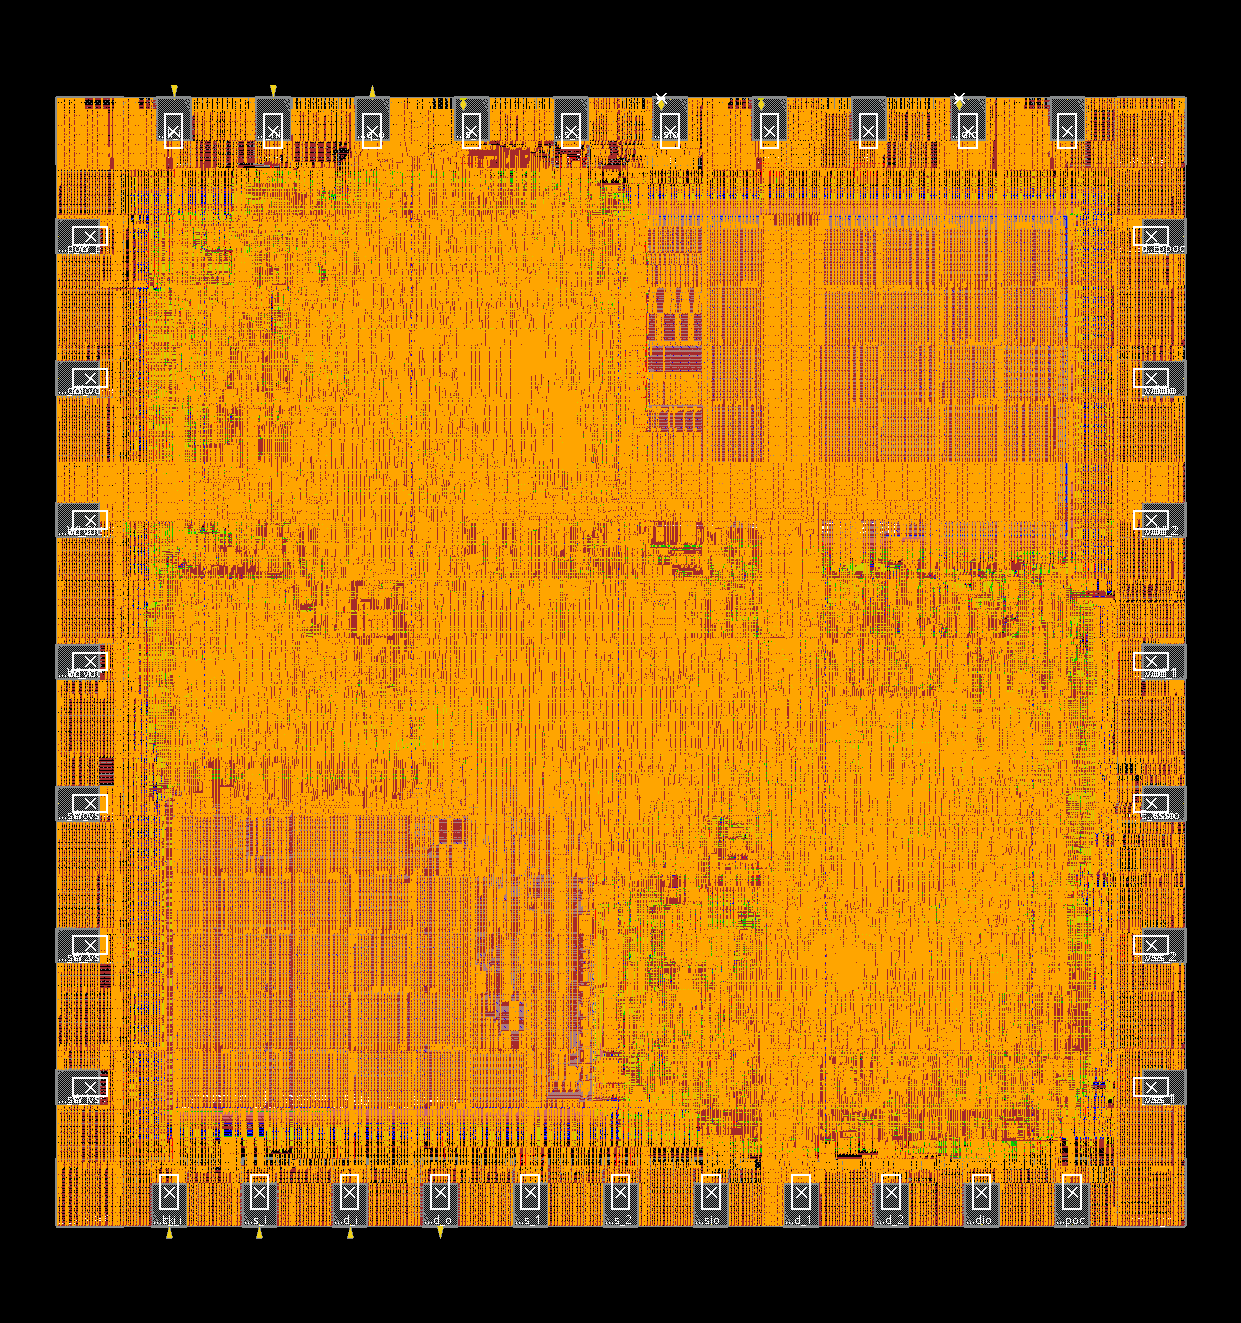
\includegraphics[width=\linewidth]{figs/5_all.png}
    \column{0.55\textwidth}
    {\small
    \begin{tabular}{@{}l l@{}}
      \toprule
      项目 & 结果 \\ \midrule
      布局 & \NLayoutName{}，利用率 \NUtil\% \\
      die（含 PAD 环） & \NDieSide{} µm $\times$ \NDieSide{} µm（预算 1950） \\
      标准单元 & \NInstances{} 个 \\
      时钟 & 50 MHz，TT 1.8 V 25 °C \\
      PrimeTime setup / hold & \NPtSetup{} ns / \NPtHold{} ns \\
      总线长 & \NWireM{} m \\
      物理检查 & 11 项全部通过 \\ \bottomrule
    \end{tabular}}
  \end{columns}
\end{frame}

\begin{frame}{签核结果}
  \normalfont{\small
  \begin{tabularx}{\linewidth}{@{}l l X@{}}
    \toprule
    检查 & 结果 & 说明 \\ \midrule
    \tabinput{data/signoff.tex}
    \bottomrule
  \end{tabularx}}
  \vspace{8pt}

  \snote{TT 单角；SRAM 接口时序由 Innovus 检查（PrimeTime 中宏为黑盒）；未做 IR/EM 与芯片级 ESD 评审。}
\end{frame}

% =====================================================================
\def\secHL{}
\section{FPGA 实现}



\begin{frame}{FPGA 实现：EGo1（XC7A35T）@ 50 MHz}
  \begin{columns}[T]
    \column{0.47\textwidth}
    \normalfont{\small
    \begin{tabularx}{\linewidth}{@{}l >{\raggedleft\arraybackslash}X@{}}
      \toprule
      项目 & 结果 \\ \midrule
      LUT & \NFpgaLut{}（\NFpgaLutPct\%） \\
      触发器 & \NFpgaFf{}（\NFpgaFfPct\%） \\
      BRAM / DSP & \NFpgaBram{} / \NFpgaDsp \\
      时钟 & 50 MHz \\
      setup / hold & \NFpgaWns{} / +\NFpgaWhs{} ns \\
      CDC Critical & 0 \\ \bottomrule
    \end{tabularx}}
    \vspace{4pt}

    \snote{Vivado 2025.2；生产配置关闭 trace；JTAG 经 FT232H，TCK 1 MHz。}
    \column{0.5\textwidth}
    \textbf{上板时发现并修复的两处 RTL 问题}
    \begin{enumerate}\small
      \item \textbf{时序}：gather 关键路径上的“是否还有下一个位置”比较改为寄存器预判，50 MHz 由 $-$0.206 ns 收敛，周期数不变
      \item \textbf{CDC}：突发协议的错误标志先在 TCK 域寄存再置位，不再直接由异步 mailbox 位驱动
    \end{enumerate}
    \snote{两处修复已并入最终 RTL，ASIC 最终版图基于修复后的代码。}
  \end{columns}
\end{frame}

\begin{frame}{FPGA 上板验证}
  \begin{columns}[c]
    \column{0.47\textwidth}
    \centering
    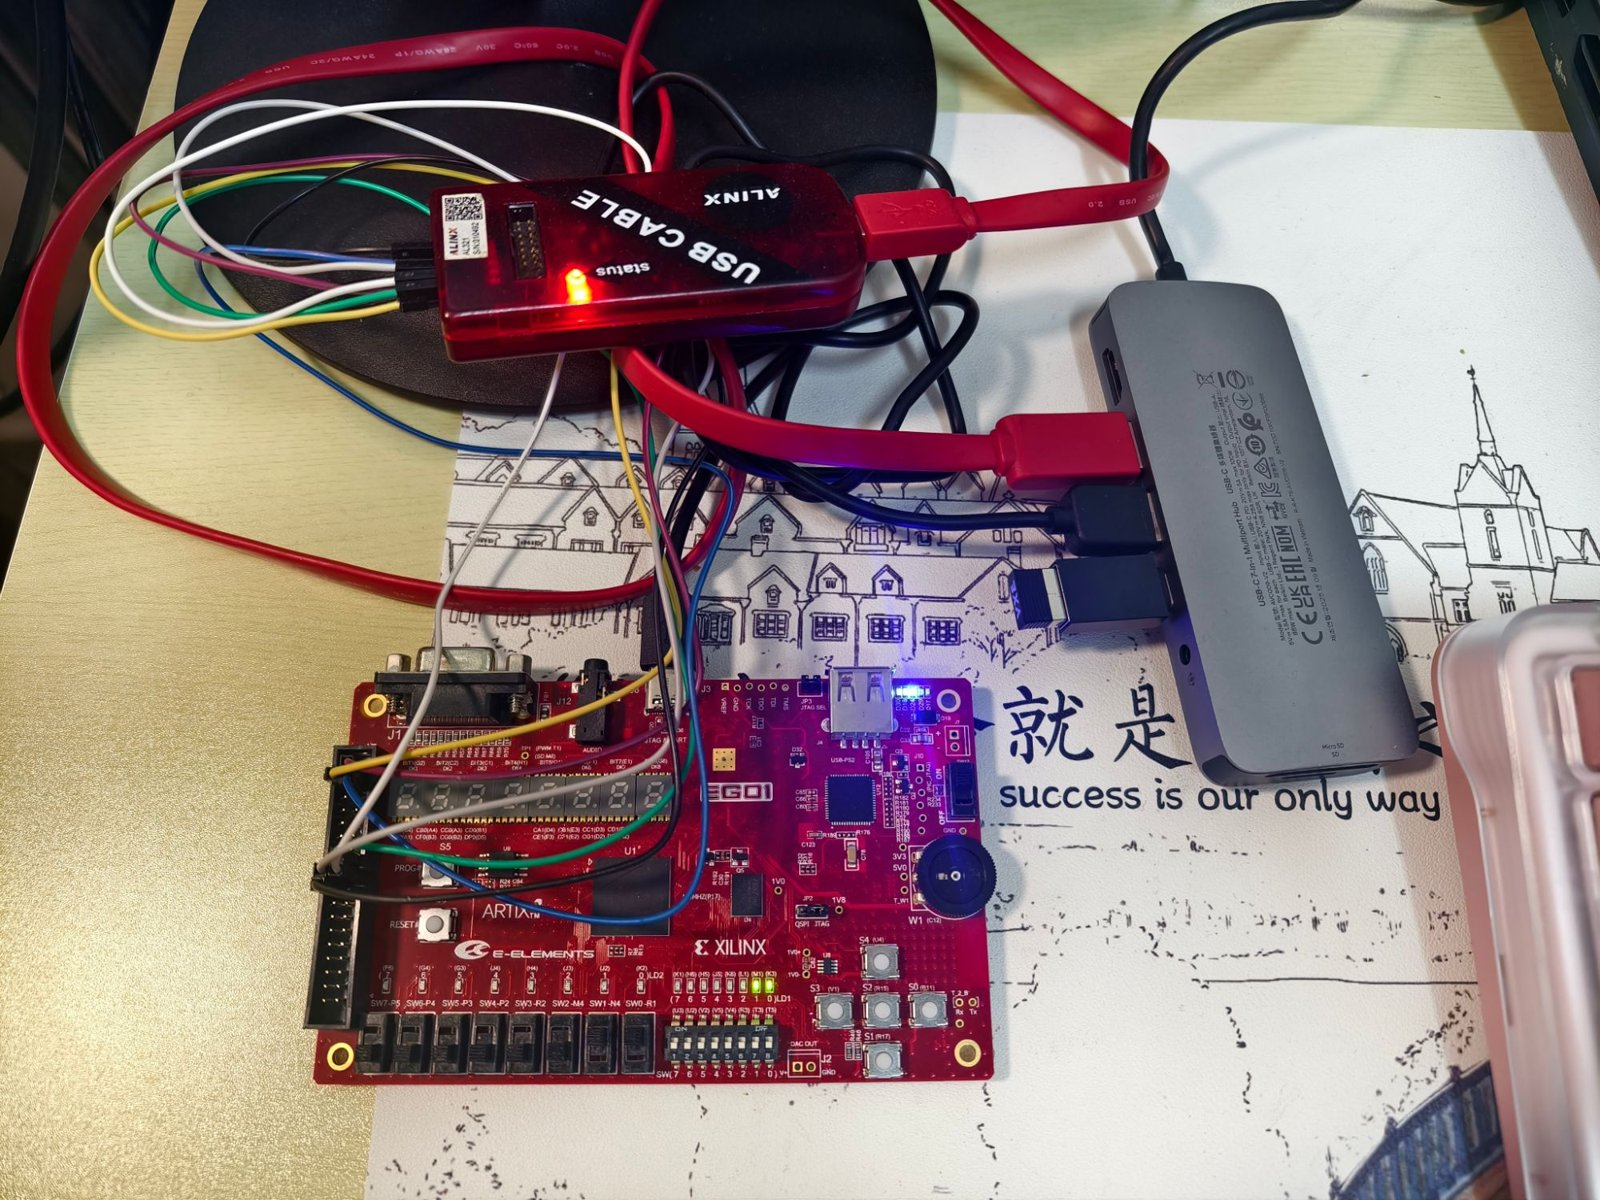
\includegraphics[width=\linewidth]{figs/fpga_board.jpg}\\
    \snote{EGo1 开发板实拍：50 MHz，外接 JTAG 驱动 NPU}
    \column{0.5\textwidth}
    \begin{itemize}\small
      \item \hl{\NFpgaModels{} 个发布模型、\NFpgaGolden{} 帧样本}，每帧冷 / 热各一次，共 \NFpgaRuns{} 次推理逐字节与参考一致
      \item 实板 24 项性能计数器与 RTL 仿真逐项相同
      \item 另有 \NFpgaConfigs{} 种模型 / 融合配置、\NFpgaFrames{} 帧推理通过；\NFpgaNegative{} 项错误注入测试通过
      \item 8 KiB 突发往返、越界恢复，忙时停 TCK、重复启动、协议复位与 watchdog 恢复均通过
      \item RTL 回归 \NFpgaRtlReg{} 项 $\times$ 4 种配置全部通过
    \end{itemize}
  \end{columns}
\end{frame}

% =====================================================================
\section{总结}



\begin{frame}{最终设计一览}
  \normalfont{\small
  \begin{tabularx}{\linewidth}{@{}l X@{}}
    \toprule
    层次 & 最终设计 \\ \midrule
    系统 & 无 CPU SoC：JTAG（逐字 + 突发 IR）$\to$ CDC mailbox $\to$ 命令控制器 $\to$ NPU；模型、激活各一颗 8 KiB SRAM \\
    NPU & 描述符驱动（16 条 $\times$ 64 B）；4$\times$8 INT4$\times$u4 阵列；双 Requant lane；向量 element 引擎 \\
    数值 & INT4 权重、u4/INT4 激活；每通道一个参数字（18 bit bias + Q8 + shift）；Requant 单次舍入 \\
    算子 & Conv（含深度可分离、1--7 矩形核、1D）、FC、Max/AvgPool、GAP、Add、ReLU、Requant；每类融合可开关 \\
    模型 & \NNumModels{} 个真实数据集模型，INT4 测试精度全部 $>$90\%（最低 \NMinAcc） \\
    芯片 & \NLayoutName{}，die \NDieSide{} µm，50 MHz；DRC / LVS / STA / LEC / SDF 门级仿真全部通过 \\
    FPGA & EGo1 @ 50 MHz；\NFpgaModels{} 个模型 \NFpgaRuns{} 次实板推理逐字节一致；两处 RTL 修复已并入最终设计 \\ \bottomrule
  \end{tabularx}}
\end{frame}

\begin{frame}{下一步}
  \begin{columns}[T]
    \column{0.48\textwidth}
    \textbf{芯片}
    \begin{itemize}\small
      \item 多角 STA，以及 IR / EM 分析（当前只有 TT 单角）
      \item hold 靠提高 Innovus 目标收敛（PrimeTime \NPtHold{} ns），多角下复查
      \item SRAM 接口时序补充独立检查（PrimeTime 中宏为黑盒）
    \end{itemize}
    \textbf{FPGA}
    \begin{itemize}\small
      \item setup 余量为 0：布线占关键路径 76\%，可提前寄存坐标 / mask 计算
      \item 补做实体按键复位、断电恢复和板上全测试集精度
    \end{itemize}
    \column{0.48\textwidth}
    \textbf{架构与模型}
    \begin{itemize}\small
      \item MAC 阵列 4$\times$8 $\to$ 8$\times$8：估计各模型周期 $-$\NArrayGainMin\%$\sim-$\NArrayGainMax\%，面积代价小（附录）
      \item 模型受 8 KiB 模型 SRAM 限制，探索更大容量或权重压缩
      \item 在真实 FT232H / OpenOCD 上实测突发协议的主机开销
    \end{itemize}
  \end{columns}
\end{frame}

{\setbeamertemplate{logo}{}
\begin{frame}
  \centering\vspace{1.2cm}
  {\Huge\textcolor{peking}{谢谢！}}\\[0.8cm]
  {\large 欢迎提问}\\[1cm]
  
\includegraphics[width=0.22\linewidth]{Figures/PKU-emblem-names.png}
\end{frame}}

% =====================================================================
\appendix
\def\secHL{}
\section{附录：设计过程}

\begin{frame}{针对性优化：计算周期 $-$\NCycleCutMin\%$\sim-$\NCycleCutMax\%}
  \begin{columns}[c]
    \column{0.58\textwidth}
    \begin{tikzpicture}
      \begin{axis}[pkubar, xbar=0pt, width=\linewidth, height=6.4cm, bar width=4pt,
          xmin=0, xlabel={每帧计算周期（千）},
          symbolic y coords={GTSRB-L,ECG-1D,HAR-1D,KWS-M,KWS-L,Fashion-CNN,MNIST-L},
          ytick={GTSRB-L,ECG-1D,HAR-1D,KWS-M,KWS-L,Fashion-CNN,MNIST-L},
          legend style={at={(0.5,1.03)}, anchor=south, legend columns=1},
          unbounded coords=discard]
        \addplot[fill=peking_gray!35, draw=none] table[x=s1, y=model] {data/stages.dat};
        \addplot[fill=peking_gold, draw=none] table[x=s2, y=model] {data/stages.dat};
        \addplot[fill=peking, draw=none] table[x=s3, y=model] {data/stages.dat};
        \legend{ABI 4 首版, + 向量 element 引擎 / 行填充, + 双 Requant lane（最终版）}
      \end{axis}
    \end{tikzpicture}
    \column{0.4\textwidth}
    \begin{enumerate}\small
      \item \textbf{向量 element 引擎}：一次读 8 个 nibble，同时更新全部通道
      \item \textbf{窄核行填充}：单通道、KW$\le$4 时每个核行补成一个 K 组，一次连续读
      \item \textbf{双 Requant lane}：相邻两个输出合并成一次写回
    \end{enumerate}
    \snote{Fashion-CNN 在第二步之后才训练完成；GTSRB-L 第二步数据未单独测量。}
  \end{columns}
\end{frame}

\begin{frame}{SRAM 摆放实验（利用率 70\%）}
  \centering
  \normalfont{\scriptsize
  \begin{tabular}{@{}l r r r r r l c@{}}
    \toprule
    布局 & die µm & PT setup & PT hold & 线长 m & 拥塞溢出 H / V & 引脚边 & 验收 \\ \midrule
    \tabinput{data/placement_table.tex}
    \bottomrule
  \end{tabular}}
  \vspace{6pt}

  \begin{itemize}\small
    \item 前两行 hold 目标 0.02 ns，其余 0.15 ns：PrimeTime 在 SPEF 上读出的 hold 比 Innovus 差约 0.1 ns，提高目标后收敛
    \item 实验用上板修复前的 RTL；最终版图在修复后的 RTL 上重新跑完整流程与签核
  \end{itemize}
\end{frame}

\begin{frame}{关键设计取舍}
  \normalfont{\footnotesize
  \begin{tabular}{@{}p{1.3cm} p{5.1cm} p{7.4cm}@{}}
    \toprule
    结论 & 选项 & 依据 \\ \midrule
    \textcolor{peking_darkgreen}{采纳} & 单次舍入 Requant、u4 激活 & 让 QAT 与整数推理一致；u4 各模型 +1--2.5 个百分点 \\
    \textcolor{peking_darkgreen}{采纳} & 每通道一个参数字（18 bit bias + Q8） & 精度不变，参数区减半 \\
    \textcolor{peking_darkgreen}{采纳} & 共享建立乘法器、增量地址、取指检查 & 约 20 个乘法器合并为 1 个，标准单元面积 $-$12.7\% \\
    \textcolor{peking_darkgreen}{采纳} & SRAM 对角摆放、提高 hold 目标 & 引脚各自面向逻辑区，拥塞最低；PrimeTime hold \NPtHold{} ns \\
    \textcolor{peking_gold}{保留选项} & TILE 8（psum 减半） & 省面积但周期增加；die 不受面积限制，默认 TILE 16 \\
    \textcolor{peking}{否决} & 第三颗 SRAM（模型 16 KiB） & 只有 8 KiB 宏可用，放进 1950 µm 余量不足 5 µm \\
    \textcolor{peking}{否决} & 模型与激活共用一颗 SRAM & 多数模型“模型 + 激活峰值”超过 8 KiB \\
    \textcolor{peking}{否决} & 硬件全局融合开关 & 融合改变描述符与张量分配，只能由编译器决定 \\
    \bottomrule
  \end{tabular}}
\end{frame}

\begin{frame}{阵列尺寸：后续方向（模型估算）}
  \centering
  \normalfont{\small
  \begin{tabular}{@{}l r r r r@{}}
    \toprule
    模型 & DW 周期占比 & 4$\times$4 & 4$\times$16 & 8$\times$8 \\ \midrule
    \tabinput{data/array.tex}
    \bottomrule
  \end{tabular}}
  \vspace{6pt}

  \begin{itemize}\small
    \item 相对当前 4$\times$8 的周期变化，由 4$\times$4 / 4$\times$8 逐层实测外推；区间两端分别假设激活读取跟得上 / 跟不上
    \item DW 层在 4$\times$4 与 4$\times$8 上周期相同：DW 每拍只算“行数”个通道，加列没有用
    \item \hl{8$\times$8} 同时加速普通卷积和 DW，psum 与结果槽不变；4$\times$16 只加速普通卷积且 psum 翻倍，die 超预算
  \end{itemize}
\end{frame}

\end{document}
